\documentclass[12pt, titlepage]{article}
\usepackage[utf8]{inputenc}
\usepackage[spanish]{babel}
\usepackage[letterpaper, margin=2.5cm]{geometry}
\usepackage{lipsum}
%\usepackage[nottoc,numbib]{tocbibind}
\usepackage{float}
\usepackage{amsmath}
\usepackage{url}
\usepackage{graphicx} 

\usepackage{listings}
\usepackage{color}
\definecolor{dkgreen}{rgb}{0,0.6,0}
\definecolor{gray}{rgb}{0.5,0.5,0.5}
\definecolor{mauve}{RGB}{253,151,31}

\lstset{frame=tb,
	aboveskip=3mm,
	belowskip=3mm,
	showstringspaces=false,
	columns=flexible,
	basicstyle={\small\ttfamily},
	numbers=none,
	numberstyle=\tiny\color{gray},
	keywordstyle=\color{blue},
	commentstyle=\color{dkgreen},
	stringstyle=\color{mauve},
	breaklines=true,
	breakatwhitespace=true,
	tabsize=3
}

\title{Reporte del primer parcial}
\author{Carlos Tonatihu Barrera Pérez \\ Profesor: Genaro Juárez Martínez \\ Teoría Computacional \\ Grupo: 2CM4 }
\date{10 de septiembre de 2016}
\begin{document}
	\maketitle
	\tableofcontents
	\newpage
	
	\section{Alfabeto}
	\subsection{Descripción del problema}
	El objetivo de esta practica es el generar las potencias del alfabeto binario $ \sum = \lbrace 0, 1 \rbrace $ desde $k=0$ hasta un $k$ seleccionado con un máximo de $k=1000$, para después guardar en un archivo todas las cadenas que se pudieron formar bajo estas condiciones, es decir: 
	\[{\sum}^{+} = {\sum}^{0}\cup{\sum}^{1}\cup{\sum}^{2}\cup\cdots\cup{\sum}^{1000}\]
	Es importante señalar que este conjunto solo es un subconjunto de $ {\sum}^{*} $ que representa todas las cadenas que se pueden formar con este alfabeto binario.
	El programa cuenta con modo manual (el usuario ingresa un $k$) y automático (genera su propio $k$).
	\subsection{Código}
	El código del programa fue realizado en C.
	\\Archivo: albafeto.h
	\begin{lstlisting}[language=C]
	//albafeto.h
	#ifndef __ALFABETO__
	#define __ALFABETO__
	
	#include <stdio.h>
	#include <stdlib.h>
	#include <time.h>
	
	static const int CONTINUAR = 1;
	int iniciar();
	int abrir_archivo(FILE **);
	int generar_palabras();
	
	#endif
	\end{lstlisting}
	Archivo: alfabeto.c
	\lstset{language=C}
	\begin{lstlisting}
	//alfabeto.c
	#include "alfabeto.h"
	
	int generar_palabras(int potencia_k) {
		FILE *archivo = NULL;
		int long_cadena;
		int i;
		int posicion;
		int *cadena_aux = NULL;
		
		abrir_archivo(&archivo);
		fputs("S = {e", archivo);
		
		for (long_cadena = 1; long_cadena <= potencia_k; long_cadena++) {
			cadena_aux = (int*) calloc(long_cadena, sizeof(int));
			if(cadena_aux == NULL) {
				printf("%s\n", "Error en el calloc");
				exit(0);
			}
			while(CONTINUAR) {
				fputc(',', archivo);
				for(i = 0; i < long_cadena; i++) {
					fputc(cadena_aux[i] + '0', archivo);
				}
				for(posicion = 0; posicion < long_cadena; posicion++) {
					cadena_aux[posicion] += 1;
					if(cadena_aux[posicion] > 1) {
						cadena_aux[posicion] = 0;
					} else {
						break;
					}
				}
				if(posicion >= long_cadena) {
					free(cadena_aux);
					break;
				}
			}
			printf("Va en 2^%d\n", long_cadena);
		}
		
		fputs("}", archivo);
		fclose(archivo);
		return 1;
	}
	
	int abrir_archivo(FILE **archivo) {
		*archivo = fopen("palabras.txt", "w");
		if (*archivo == NULL) {
			printf("%s\n", "No se pudo abrir");
			exit(0);
		}
		return 1;
	}
	
	\end{lstlisting}
	Archivo: main.c
	\begin{lstlisting}[language=C]
	//albafeto.h
	#include "main.c"
	
	int iniciar();
	int menu();
	int menu_continuar();
	int random_potencia_k();
	
	int main(int argc, char const *argv[]) {
		printf("%s\n", "***************Alfabeto****************");
		iniciar();
		return 0;
	}
	
	int iniciar() {
		srand(time(NULL));
		int continuar = 1;
		int potencia_k = 1;
		int manual = 1;
		while(continuar) {
			manual = menu();
			if (manual == 1) {
				printf("%s\n", "Ingresa el valor de k: ");
				scanf("%d", &potencia_k);
			} else if (manual == 2) {
				potencia_k = random_potencia_k();
			} else {
				break;
			}
			printf("El valor de k es: %d\n", potencia_k);
			generar_palabras(potencia_k);
			printf("%s\n", "Cadenas guardadas en el archivo palabras.txt");
			continuar = menu_continuar();
		}
		printf("\n%s\n", "Saliendo...");
		return 1;
	}
	
	int menu_continuar() {
		int opcion;
		printf("Intentar otra vez?\nSi = 1 NO = 0\n");
		scanf(" %d", &opcion);
		return opcion;
	}
	
	int menu() {
		int opcion;
		printf("Que quieres hacer?\n1.-Manual\n2.-Automatico\n3.-Salir\n");
		scanf(" %d", &opcion);
		return opcion;
	}
	
	int random_potencia_k() {
		//numero = rand () % (N-M+1) + M;
		// Cambiar el valor del random k a 1000
		int potencia_k = 1 + rand() % (10 + 1 - 1);
		return potencia_k;
	}
	\end{lstlisting}
	\subsection{Pruebas}
	Las pruebas están divididas en modo automático y manual, en ambos dada una k se generan todas las cadenas de longitud 1 hasta $k$.
	\\\\
	{\large Modo automático.}
	\begin{figure}[H]
		\begin{center}
			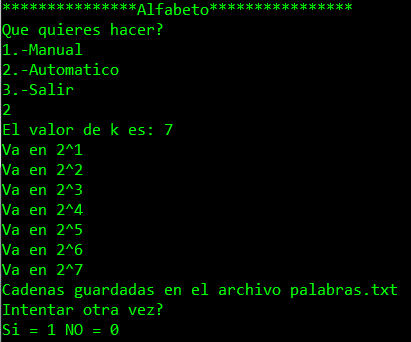
\includegraphics[width=7cm, height=7cm]{img/automatico-alfabeto.png}
			\caption{Alfabeto con k = 7.}
			\label{fig:alfabeto1}
		\end{center}
	\end{figure}
	\begin{figure}[H]
		\begin{center}
			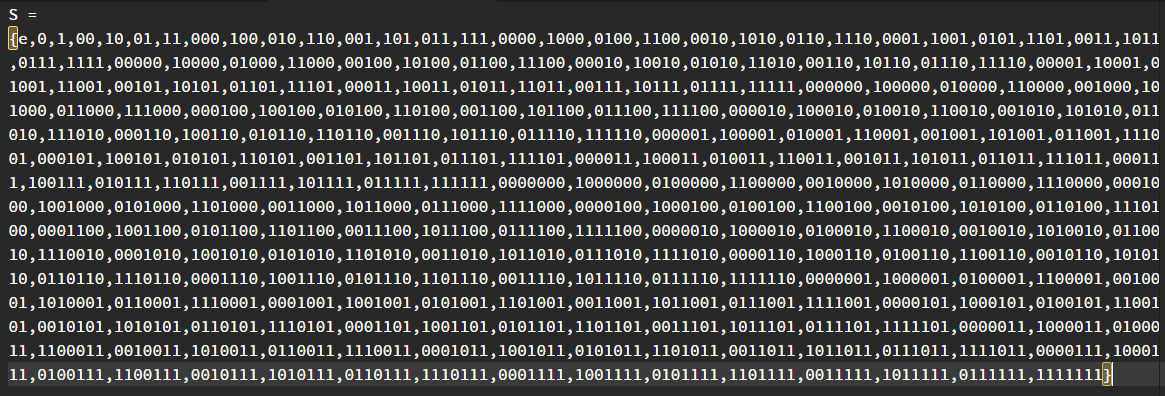
\includegraphics[width=\linewidth, height=8cm]{img/automatico-alfabeto-salida.png}
			\caption{Archivo generado.}
			\label{fig:alfabeto2}
		\end{center}
	\end{figure}
	{\large Modo manual.}
	\begin{figure}[H]
		\begin{center}
			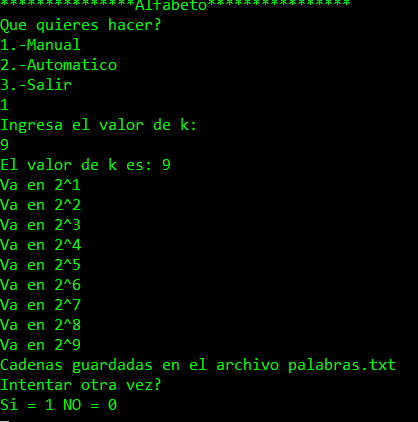
\includegraphics[width=7cm, height=7cm]{img/manual-alfabeto.png}
			\caption{Alfabeto con k = 9.}
			\label{fig:alfabeto3}
		\end{center}
	\end{figure}
	\begin{figure}[H]
		\begin{center}
			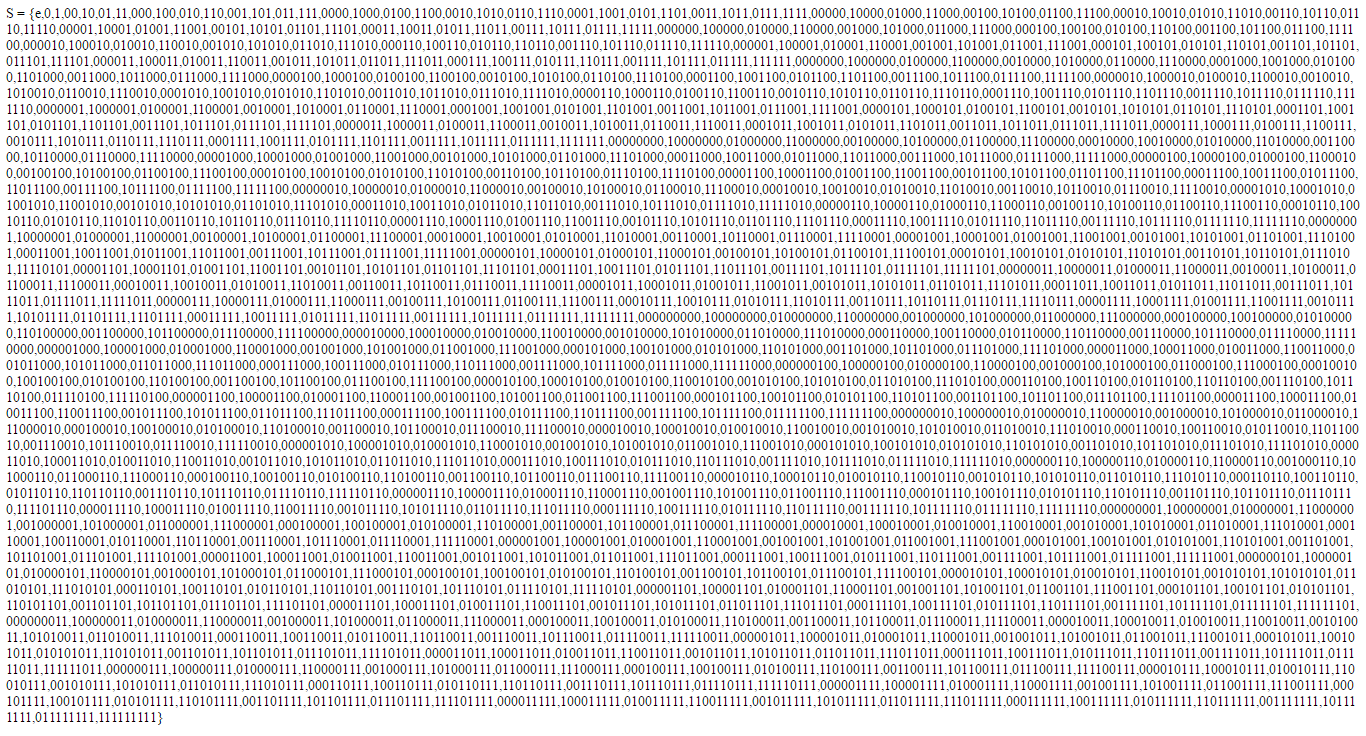
\includegraphics[width=\linewidth, height=12cm]{img/manual-alfabeto-salida.png}
			\caption{Archivo generado.}
			\label{fig:alfabeto4}
		\end{center}
	\end{figure}
	
	\section{Números primos}
	\subsection{Descripción del problema}
	Desarrollar un programa que encuentre todos los números primos en el intervalo $0 \leq n \leq 1000$ imprimirlos en pantalla junto con su representación en binario ademas de contar la cantidad de ceros y unos en dicho numero, finalmente guarda los números primos en su forma binaria en un archivo txt.
	Cuenta con modo manual (el usuario ingresa un numero n) y automático (el programa utiliza un $n$ aleatorio).
	\subsection{Código}
	El código del programa fue realizado en Python 3.5.
	\subsection{Pruebas}
	Las pruebas están divididas en modo automático y manual.
	{\large Modo automático.}
	{\large Modo manual.}
	\begin{figure}[ht]
		\begin{center}
			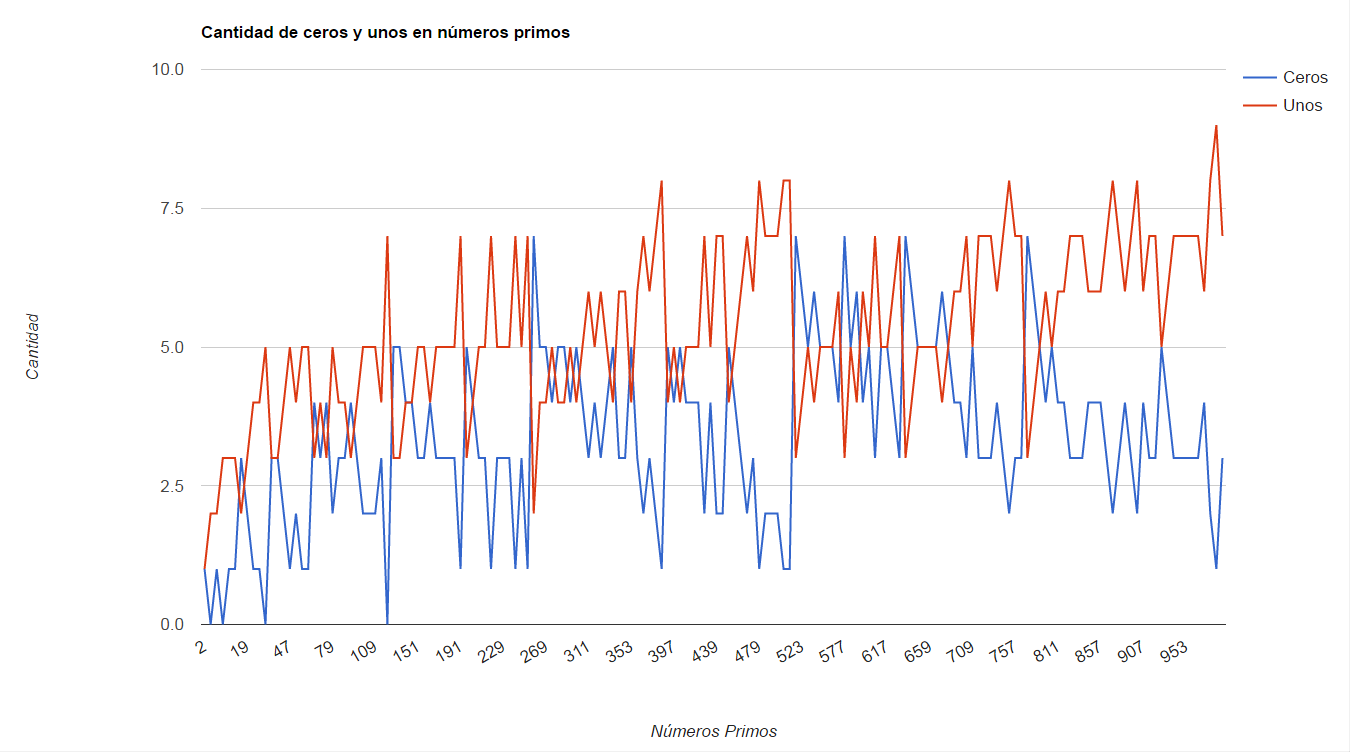
\includegraphics[width=\linewidth, height=7cm]{img/primos.png}
			\caption{Cantidad de ceros y unos encontrados entre 1 y 1000.}
			\label{fig:grafica}
		\end{center}
	\end{figure}
	
	\section{AFD Palabras con terminación 'ere'}
	\subsection{Descripción del problema}
	Desarrollar un autómata finito determinista capaz de encontrar las palabras con terminación 'ere' ya sea leyendo un archivo txt o en una linea de texto que el usuario ingresa, y que dichas palabras se muestren en pantalla y en el caso del archivo de texto imprimir la linea y el numero de palabra (por linea) en el que fue encontrada dicha palabra.
	Es importante señalar que todo aquello que no es un símbolo del alfabeto ingles, $ \sum =\lbrace a, b, ..., z, A, B, ..., Z \rbrace $, es tomado como un espacio. Además, debe tener una opción para visualizar el siguiente diagrama.
	\begin{figure}[ht]
		\begin{center}
		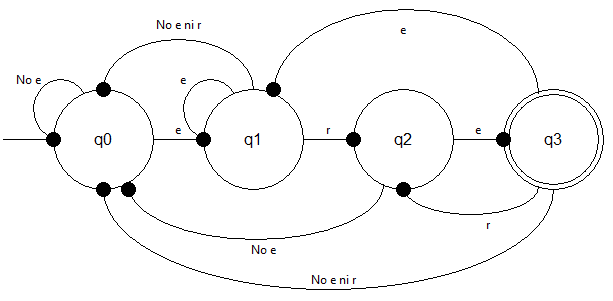
\includegraphics[width=14cm, height=7cm]{img/ere.png}
		\caption{Diagrama de transiciones del autómata 'ere'.}
		\label{fig:diagrama1}
		\end{center}
	\end{figure}
	\subsection{Código}
	El código fue realizado en Python 3.5.
	\subsection{Pruebas}
	Pruebas de las opciones del menú.
	{\large Modo automático.}
	{\large Modo manual.}
	{\large Diagrama.}
	
	\section{AFD Paridad en números binarios}
	\subsection{Descripción del problema}
	Diseñar y programar un autómata finito determinista que acepte el lenguaje:
	\[ L = \lbrace w \mid w \text{ tiene un número par de ceros y un numero par de unos} \rbrace \text{\cite{LIBRO}}\] 
	Es decir, los números binarios de entrada se generan de manera automática (cadena de longitud $n \mid 1\leq n \leq 1000$) o manual y después se imprime si es una cadena valida o no y en ambos casos imprimir su historia. Ademas, mostrar el siguiente diagrama.
	\begin{figure}[ht]
		\begin{center}
			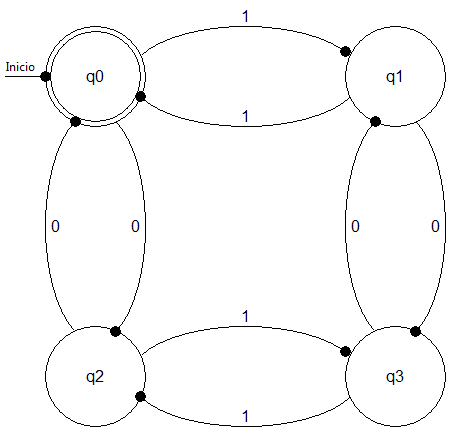
\includegraphics[width=7cm, height=7cm]{img/paridad.png}
			\caption{Diagrama de transiciones del autómata. \cite{LIBRO}}
			\label{fig:diagrama2}
		\end{center}
	\end{figure}
	\subsection{Código}
	El código fue realizado en Python 3.5.
	\subsection{Pruebas}
	Pruebas de las opciones del menú.
	{\large Modo automático.}
	{\large Modo manual.}
	{\large Diagrama.}
	
	\section{Protocolo de transmisión}
	\subsection{Descripción del problema}
	Desarrollar un programa que genere 50 cadenas de 32 caracteres que sean guardadas en un archivo, para después ser evaluadas por un autómata, en este caso el autómata de paridad binaria y guardar las cadenas binarias en otro archivo, siguiendo el siguiente diagrama.
	\begin{figure}[ht]
		\begin{center}
			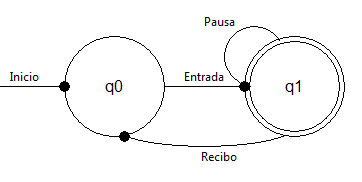
\includegraphics[width=10cm, height=5cm]{img/protocolo.png}
			\caption{Diagrama de transiciones del autómata. \cite{WEB}}
			\label{fig:diagrama3}
		\end{center}
	\end{figure}
	\subsection{Código}
	El código fue realizado en Python 3.5.
	\subsection{Pruebas}
	Pruebas de las opciones del menú.
	{\large Modo automático.}
	{\large Diagrama.}
	
	\section{AFND Números binarios con terminación '01'}
	\subsection{Descripción del problema}
	Desarrollar un autómata finito no determinista, que acepte todas y sólo las cadenas formadas por ceros y unos que terminan en 01. Asimismo, imprimir la tabla de transiciones (historia) y que la entrada de cadenas sea de forma manual o automática, la cadena automática debe de tener una longitud $n \mid 1  \leq n \leq 1000$. Y que contenga la opción de mostrar el siguiente diagrama.
	\begin{figure}[ht]
		\begin{center}
			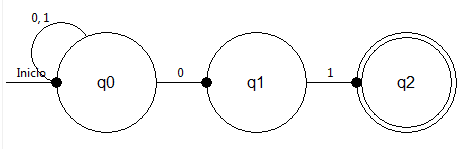
\includegraphics[width=12cm, height=4cm]{img/cero-uno.png}
			\caption{Diagrama de transiciones del autómata. \cite{LIBRO}}
			\label{fig:diagrama4}
		\end{center}
	\end{figure}
	
	\subsection{Código}
	El código fue realizado en Python 3.5.
	\subsection{Pruebas}
	Pruebas de las opciones del menú.
	{\large Modo automático.}
	{\large Modo manual.}
	{\large Diagrama.}
	
	\bibliography{bibliografia} 
	\bibliographystyle{ieeetr}
\end{document}